%%%%%%%%%%%%%%%%%%%%%%% file typeinst.tex %%%%%%%%%%%%%%%%%%%%%%%%%
%
% This is the LaTeX source for the instructions to authors using
% the LaTeX document class 'llncs.cls' for contributions to
% the Lecture Notes in Computer Sciences series.
% http://www.springer.com/lncs       Springer Heidelberg 2006/05/04
%
% It may be used as a template for your own input - copy it
% to a new file with a new name and use it as the basis
% for your article.
%
% NB: the document class 'llncs' has its own and detailed documentation, see
% ftp://ftp.springer.de/data/pubftp/pub/tex/latex/llncs/latex2e/llncsdoc.pdf
%
%%%%%%%%%%%%%%%%%%%%%%%%%%%%%%%%%%%%%%%%%%%%%%%%%%%%%%%%%%%%%%%%%%%


\documentclass[runningheads,a4paper]{llncs}

\usepackage{amssymb}
\setcounter{tocdepth}{3}
\usepackage{graphicx}
\usepackage{hyperref}
\usepackage{amsmath}
\usepackage{listings}

\usepackage{tikz}
\usetikzlibrary{positioning,arrows,shapes.geometric,
	matrix,shapes.symbols,decorations.pathreplacing}

\usepackage{subcaption}
\captionsetup{compatibility=false}

\usepackage{booktabs}

\usepackage[utf8]{inputenc}
\usepackage[T1]{fontenc}
\usepackage{lmodern}

\usepackage{url}
\urldef{\mailsa}\path|loic_tetrel@yahoo.fr|
\newcommand{\keywords}[1]{\par\addvspace\baselineskip
	\noindent\keywordname\enspace\ignorespaces#1}

\begin{document}
	
	\mainmatter  % start of an individual contribution
	
	% first the title is needed
	\title{Dimensionality reduction}
	
	% a short form should be given in case it is too long for the running head
	\titlerunning{Dimensionality reduction}%
	
	% the name(s) of the author(s) follow(s) next
	%
	% NB: Chinese authors should write their first names(s) in front of
	% their surnames. This ensures that the names appear correctly in
	% the running heads and the author index.
	%
	\author{Loïc Tetrel}
	%
	\authorrunning{Dimensionality reduction}
	% (feature abused for this document to repeat the title also on left hand pages)
	
	% the affiliations are given next; don't give your e-mail address
	% unless you accept that it will be published
	%\institute{******************************************\\
	\institute{}
	
	%
	% NB: a more complex sample for affiliations and the mapping to the
	% corresponding authors can be found in the file "llncs.dem"
	% (search for the string "\mainmatter" where a contribution starts).
	% "llncs.dem" accompanies the document class "llncs.cls".
	%
	
	\toctitle{Dimensionality reduction}
	
	\maketitle

	\keywords{Eigen vectors, eigen values}

	\section{Introduction}\label{introduction}
	In a machine learning, it is really important to choose wisely the features, which will abstract the meaning of the image. Your algorithm will be faster if you have less features to analyze, and will have more meaning.
	\par In an image containing thousands of thousands pixels, you can use features like SIFT \cite{lowe1999object}, Harris corner detection \cite{harris1988combined}, parameters from a model where your pixels come from... The process of comparing a feature with another one is called \textbf{selection}. Another way to extract good feature is \textbf{projection} and this is the purpose of this article.

	\section{Projection of features}\label{theory}
	The key idea is to abstract all your data in a new dimension space. This dimension space will summarize the information in a new way. One widely known technic to do that is called principal component analysis (PCA) projection. Discovered by Pearson \cite{kpfrs1901lines} and developped by \cite{hotelling1933analysis}, the goal is to extract the principal axes from a population, which has the largest variation. Imagine the cloud in figure, using the raw data will be more challenging than working with the projections in a new dimension. For this particular example, you can imagine to apply a basic bayesian based classification with gaussian prior.
	
	\begin{figure}
		\centering
		\includegraphics[width=0.75\textwidth]{Figures/pcaProj}
		\\ \parbox{0.75\textwidth}{\caption[pcaProj]{Projections }\label{fig:pcaProj}} 
	\end{figure}
	\subsection{Theory}
	
	VOIR TP2 MACHINE LEARNING CHERIET avec eigen implementé
	
	\section{Eigen faces}
	Face recognition task is really hard because you need to process images with hundred of thousands pixels. This is why
	PCA has been intensively used in this area, for its capability to summarize well the data.
	\par
	Imagine some squared images $M$ characterized by $N^2$ pixel, encoded in a vector $[1,N^2]$. These images differs from the average image $\Psi=\frac{1}{M}\sum_{n=1}^M\Gamma_n$ by the matrix $A=\Gamma-\Psi$.
	Principal component analysis will find the $M$ orthogonal vectors $v_M$ that maximizes the variance $\lambda_k$ along each vector, i.e. we search the eigen vectors $v_k$ and eigen values $\lambda_k$ of the covariance matrix $C$ :
	\begin{equation}
	C=A^tA
	\end{equation}
	Because the covariance $C$ is $N^2$ by $N^2$, the snapshot method \cite{turk1991face} says that the best $\lambda_k$ are the same as $C=AA^t$ which is $M$ by $M$. 
	Usually the training set is much lower than the number of dimension $(M<<N^2)$ so this allowed us to compute $v_M$ and $\lambda_k$ much faster. The mapping from the pixel-space to the face-space and is given by :
	\begin{equation}
	u=v^tA
	\end{equation}
	
	The matrix $u$ is called the eigen faces and is $M$ by $N^2$.
	\section{Reconstruction}
	\section{Conclusion}
	Look at http://vis-www.cs.umass.edu/lfw/results.html
	for state of the art face recognition
	\subsection*{Acknowledgment}
	Thanks
	
	{\small
		\bibliographystyle{splncs03}
		\bibliography{article}
	}
	
\end{document}

